%=====================================================================
\section{Metodología: datos y modelos}

La metodología sigue las etapas de CRISP-ML(Q) \cite{Studer2021}. Esta sección cubre la comprensión y preparación de los datos (etapa 2) y la elección de los modelos (etapa 3). El protocolo de evaluación completo se presenta en la Entrega 3.

\subsection{Construcción del dataset}

Se minó un clon completo de \texttt{torvalds/linux} con una sola pasada de \texttt{git log} sobre la rama principal, sin commits de fusión, desde 2014. Los años 2014--2018 solo sirven para calcular la experiencia de los autores. Por cada commit se extraen el \emph{numstat} del diff, los trailers del mensaje y las fechas. Las referencias \texttt{Fixes:} (prefijos de al menos 8 caracteres hexadecimales) se resuelven contra el historial: el 9,4\,\% que no se resuelve apunta a commits anteriores a 2014 o a otros árboles.

\textbf{Etiqueta.} Un commit es \emph{riesgoso} si algún commit posterior de la rama principal lo cita con \texttt{Fixes:} en 90 días o menos. Los commits con menos de 90 días de observación a la fecha de corte quedan \emph{censurados} y se excluyen (\cifCensurados{} commits), porque su etiqueta negativa todavía no es definitiva \cite{Falessi2022,Cabral2019}.

\textbf{Anonimización.} Nombre y correo del autor se reemplazan por un SHA-256 con sal. No se publica el texto de los mensajes.

La Tabla~\ref{tab:ficha} resume la ficha del dataset y su validación con los criterios D1--D7 del enunciado. Las \cifNVariables{} variables candidatas son las familias clásicas de JIT \cite{Kamei2013}:
\begin{itemize}
\item tamaño: líneas añadidas y borradas, archivos y binarios;
\item difusión: directorios de primer nivel y subsistemas;
\item revisión: \texttt{Reviewed-by}, \texttt{Acked-by}, \texttt{Tested-by}, \texttt{Reported-by}, \texttt{Signed-off-by}, \texttt{Co-developed-by} y \texttt{Link};
\item propósito: si trae su propio \texttt{Fixes:}, si pide backport a \emph{stable}, si el asunto menciona \emph{fix} y la longitud del asunto;
\item experiencia: commits previos del autor, en total y en el subsistema, y días desde su primer commit;
\item momento: hora y día de la semana.
\end{itemize}
Todas se conocen al integrar el commit.

\begin{table}[!t]
\caption{Ficha del dataset y verificación D1--D7}
\label{tab:ficha}
\centering\footnotesize
\begin{tabularx}{\columnwidth}{@{}l Y@{}}
\toprule
\cabecera & \textbf{Valor}\\
\midrule
Fuente & Clon de \texttt{torvalds/linux}, rama principal, GPL-2.0\\
Periodo & 2019-01-01 a 2026-07-31\\
D1 Tamaño & \cifCommits{} commits no censurados: \cifDesarrollo{} de desarrollo (2019--2025) y \cifPrueba{} de prueba (2026)\\
D2 Objetivo & Riesgoso (binaria): \cifPositivosDesarrollo{} positivos en desarrollo, prevalencia anual entre \cifPrevMin{} y \cifPrevMax{}\\
D3 Calidad & Sin faltantes ni hashes duplicados; colas pesadas (hasta 730\,092 líneas en un commit); 3 fechas de autor corruptas\\
D4 Estructura & Eventos irregulares ordenados por fecha del committer; \cifAutores{} autores y \cifSubsistemas{} subsistemas\\
D5 Disponibilidad & Solo información del propio commit y del pasado del autor\\
D6 Licencia y ética & Metadatos públicos; autores anonimizados\\
D7 Documentación & Diccionario de las \cifNVariables{} variables en el anexo\\
\bottomrule
\end{tabularx}
\end{table}

\subsection{Análisis exploratorio}

Hay tres hallazgos que guían el diseño:
\begin{itemize}
\item \textbf{La prevalencia depende de la adopción de \texttt{Fixes:}.} Antes de 2019 crece año a año (Fig.~\ref{fig:eda}), porque cada vez más correcciones usan el trailer, no porque el código empeore. Desde 2019 se estabiliza entre \cifPrevMin{} y \cifPrevMax{}, y por eso el entrenamiento empieza el 1 de enero de 2019. En 2026 baja a \cifPrevAnioVeintiseis{}.
\item \textbf{El tamaño es la señal dominante y no es lineal.} La prevalencia pasa de \cifPrevQunoAdd{} en el quintil más pequeño de líneas añadidas a \cifPrevQcincoAdd{} en el más grande, con una distribución de colas muy pesadas.
\item \textbf{Hay deriva en las covariables antes de 2026.} El número medio de \texttt{Reviewed-by} por commit sube de \cifReviewedIni{} (2019) a \cifReviewedFin{} (2025), y la fracción de commits que son correcciones, de \cifFixIni{} a \cifFixFin{}.
\end{itemize}
En correlación de Spearman, dos pares son casi redundantes: directorios de primer nivel y subsistemas (0,97), y experiencia y antigüedad del autor (0,73). Por eso el modelo difuso usa solo uno de cada par.

\begin{figure}[!t]
\centering
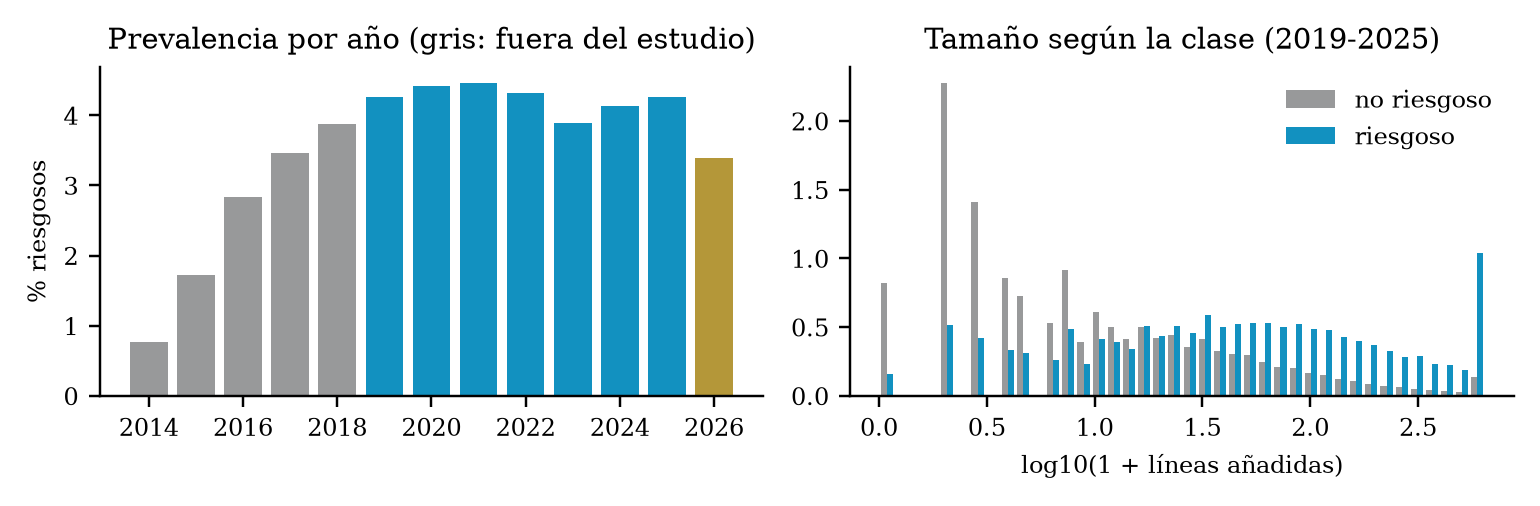
\includegraphics[width=\columnwidth]{../../resultados/e2/prevalencia_y_tamano.png}
\caption{Izquierda: prevalencia de commits riesgosos por año (en gris, los años fuera del estudio). Derecha: distribución del tamaño por clase en 2019--2025.}
\label{fig:eda}
\end{figure}

\subsection{Modelos y su papel}

La Tabla~\ref{tab:modelos} resume los modelos. Las dos referencias clásicas cubren dos extremos. La regresión logística es el estándar de JIT y es difícil de superar con partición temporal \cite{Kamei2013,Zeng2021}. El \emph{gradient boosting} \cite{Friedman2001} da la cota alta de una caja negra sobre las mismas variables.

\begin{table}[!t]
\caption{Modelos comparados}
\label{tab:modelos}
\centering\footnotesize
\begin{tabularx}{\columnwidth}{@{}l l Y@{}}
\toprule
\cabecera \textbf{Modelo} & \textbf{Papel} & \textbf{Justificación}\\
\midrule
Clase mayoritaria & Trivial & Su AUC-PR es la prevalencia: el piso\\
Reg.\ logística & Clásica & Estándar de JIT \cite{Kamei2013}; $\log(1+x)$ y estandarización\\
\emph{Gradient boosting} & Clásica fuerte & Cota alta sin restricción de interpretabilidad \cite{Friedman2001}\\
Difuso-evolutivo & Propuesto & $\le$15 reglas legibles; vértices y reglas ajustados con un AG\\
Difuso sin evolución & Variante de control & Mismas reglas iniciales, sin AG: mide el aporte de la evolución\\
\bottomrule
\end{tabularx}
\end{table}

\textbf{Qué propiedad de los datos aprovecha el modelo propuesto.} El riesgo crece por umbrales con el tamaño y la difusión, se modula con la revisión y la experiencia, y las variables tienen colas muy pesadas. Una partición difusa sobre la escala de cuantiles captura esos umbrales sin depender de la escala. Las reglas con pocos antecedentes capturan las interacciones que un mantenedor reconoce, por ejemplo ``si el cambio es grande y toca varios subsistemas''. El modelo usa 10 variables fijadas antes de ver resultados: líneas añadidas y borradas, archivos, subsistemas, \texttt{Reviewed-by}, \texttt{Signed-off-by}, si es corrección, si va a \emph{stable} y la experiencia del autor, en total y en el subsistema.

\subsection{Clasificador difuso-evolutivo}

Cada variable $x_j$ se lleva a $z_j\in[0,1]$ con su función de distribución empírica, estimada solo con el entrenamiento. Sobre $z_j$ se definen tres términos (bajo, medio, alto) que forman una partición de Ruspini \cite{Ruspini1969} con vértices $a_j<b_j<c_j$: bajo vale 1 hasta $a_j$ y cae a 0 en $b_j$; medio es el triángulo $(a_j,b_j,c_j)$; alto sube de 0 en $b_j$ a 1 en $c_j$. Una regla $r$ tiene hasta tres antecedentes y un peso $w_r\in[0,1]$:
\begin{equation}
\mu_r(\mathbf{x})=\prod_{(j,t)\in A_r}\mu_{jt}(z_j),\qquad
s(\mathbf{x})=1-\prod_{r}\bigl(1-w_r\,\mu_r(\mathbf{x})\bigr),
\end{equation}
es decir, t-norma producto y O probabilístico entre reglas. El puntaje $s$ ordena los commits por riesgo.

El ajuste sigue el enfoque Pittsburgh de los sistemas difusos genéticos \cite{Herrera2008,Ishibuchi2001}: cada individuo codifica todos los vértices y la base completa de reglas (activación, antecedentes, términos y pesos). La aptitud es el AUC-PR de entrenamiento, que es la métrica adecuada con clases desbalanceadas \cite{Saito2015}, menos una penalización por el número de antecedentes. Los operadores son:
\begin{itemize}
\item selección por torneo y elitismo;
\item cruce uniforme, que hereda cada regla completa;
\item mutación gaussiana de vértices y pesos, y mutación aleatoria de antecedentes y términos.
\end{itemize}

La variante sin evolución fija los vértices en los cuantiles $(0{,}2;\,0{,}5;\,0{,}8)$ y elige reglas de 1 o 2 antecedentes de forma voraz, por su confianza difusa, mientras mejore el AUC-PR. Esa misma solución siembra la población inicial del AG. Así, la diferencia entre ambas variantes aísla el aporte de la evolución.
